\chapter{Dynamic reconfigurable configuration method}  \label{chap:study}
%Experiments on Localization Reliability and Improvement

Having studied the estimator's behavior for several different configurations and conditions, there is still uncertainty about the best performance it can achieve. In the considered system, the hydrophone configuration has a decisive role on the achieved precision, as demonstrated. Therefore, a way to optimize the system's estimation would be to choose, for each position of the acoustic source, the configuration that returns the best estimation and thus the one that should be employed.

In a field scenario where a vehicle is searching for an acoustic transmitter, as it is navigating and readjusting its trajectory, the relative direction that is being estimated in real time is changing. Therefore, the system's performance can vary and arises the necessity of having different angles of vision from the hydrophones to the target. To resolve this issue, the proposed method assumes that the used USBL system integrates more than four hydrophones placed in known positions. This way, it is possible to dynamically reconfigure which four hydrophones are used at a time leading to an estimation that is optimal for the available sensors. 

Another possibility is to determine through the same techniques which configuration of four hydrophones, tested in various positions along the vehicle, is the overall best for short and long range estimation. This can lead to a moderate compromise of the estimate accuracy, however decreases the number sensors that are employed and therefore the cost of the system.

This chapter is dedicated to explaining the methodological approach, the main findings and conclusions that were driven from the formulated dynamic reconfigurable configuration method.

\note{descrever mais detalhadamente os temas que vao ser abordados no capitulo}

\section{Monte Carlo Approach} \label{sec:config-perf}

The developed algorithm serves as a tool to determine which is the best available hydrophone configuration for a certain target position. This approach uses a Monte Carlo method which is useful to solve problems that are deterministic in nature through repetition and application of random parameters. Additionally, it makes use of the developed estimator, which is comprehensively explained in \ref{subsec:estimator}, to estimate the target position for each sensor configuration.
		
For this experiment, it is considered a total of nine hydrophones, whose positions are contained in $matrix_{r_{i}}$, defined by table \ref{tab:config-9h}. Each column expresses the coordinates of each hydrophone, $r_i$, where the value of $x_i$ is in the first row, the value of $y_i$ in the second row and the value of $z_i$ in the third row. Additionally, it is assumed $q = 0.1$, $w = 0.1$ and $e = \frac{ \sqrt{2}}{2} * w$.

\begin{table}[!htbp] %use H to adjust
	\begin{center}
		\begin{tabular}{c | c c c c c c c c c}
			\toprule
			& r1 & r2 & r3 & r4	& r5 & r6 & r7 & r8	& r9 \\ \hline 
			\multirow{1}{0.5em}{x} 
			& q & 0 & 0 & 0 & 0 & 0 & 0 & 0 & 0\\
			\midrule 
			\multirow{1}{0.5em}{y} 
			& 0 & 0 & 0 & w & -w & e & e & -e & -e\\
			\midrule 
			\multirow{1}{0.5em}{z} 
			& 0 & w & -w & 0 & 0 & e & -e & e & -e \\
			\bottomrule 
		\end{tabular}
		\caption{Position coordinates for the implementation using 9 hydrophones}
		\label{tab:config-9h}
	\end{center}
\end{table}

These positions are arranged so that they can mimic a possible deployment in an AUV, as represented in figure \ref{fig:9h-config}, where hydrophone $r_1$ is placed in front of the vehicle and hydrophones $r_2$ to $r_9$ form a circle with a $10 cm$ radius around the vehicle.

\begin{figure}[!htbp]
	
	\makebox[\textwidth][c]{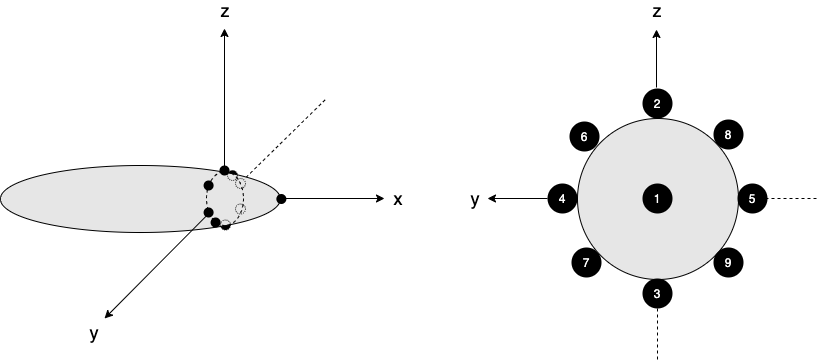
\includegraphics[width=0.8\textwidth]{figures/9h-config}}
	\captionsetup{justification=centering,margin=2cm}
	\caption{Hydrophone positions for the implementation using 9 hydrophones}
	\label{fig:9h-config}
\end{figure}

Since the used configuration has to be three dimensional, it is defined that hydrophone $r_1$ always integrates the configuration as it is the only one that covers a third dimension. Accordingly, the number of possibilities is combinations of three out of eight, $C(8,3)$, making up a total of 56 combinations. Each of these configurations are associated with a number from 1 to 56 and the hydrophones that integrate each of them are outlined in table \ref{tab:long} for consultation when necessary.

Having the system presented, the algorithm will be explained next. For the sake of clarity, the algorithm was outlined in pseudo code and separated into two main parts, where \ref{alg:alg1} is integrated in \ref{alg:alg2}.

\begin{algorithm}
	\setstretch{1.3} 	%increase space between lines
	%\algsetup{linenosize=\scriptsize} 	%adapts font size
	\scriptsize		%makes it smaller, idk
	\caption{Determines the average azimuth errors, elevation errors and MSE for a set of hydrophone configurations}
	\label{alg:alg1}
	\begin{algorithmic}[1]
		\FOR{\texttt{all k configurations}} %k = 1 \textbf{to} n\_config
		\FOR{\texttt{all i estimation repetition}} %i = 1 \textbf{to} accum\_samples
		\STATE\texttt{$estimator(s, config(k), error)$}
		\COMMENT{returns estimate in Cartesian and spherical coordinates}
		\STATE \texttt{accum\_estimate(i) $\gets$ result of the estimator in each repetition} 
		\STATE \texttt{accum\_error\_azimuth(i) $\gets$ azimuth error in each repetition} 
		\STATE \texttt{accum\_error\_elevation(i) $\gets$ elevation error in each repetition} 
		\ENDFOR
		\STATE $mean\_estimate \gets \dfrac{accum\_estimate}{accum\_samples}$
		%\newline
		%\STATE \texttt{Compute the mean and standard deviation of accum\_error\_elevation and accum\_error\_azimuth}
		\STATE
		\STATE $deviation\_azimuth(config) = std(accum\_error\_azimuth);$
		\STATE $deviation\_elevation(config) = std(accum\_error\_elevation);$
		%\newline
		\STATE $error\_azimuth(config) = mean(accum\_error\_azimuth);$
		\STATE $error\_elevation(config) = mean(accum\_error\_elevation);$
		\STATE
		\STATE $mse(config) = \sqrt{\rule{0pt}{8pt}error\_azimuth(config)^{2} + error\_elevation(config)^{2}};$
		%				\newline
		%				\IF {\texttt{$min\_mse > mse(config)$}} 
		%				\STATE	$min\_mse\_config = config$  
		%				\ENDIF
		%				\IF {\texttt{$min\_error\_azimuth > deviation\_azimuth(config)$}} 
		%				\STATE $min\_azimuth\_config = config$  
		%				\ENDIF
		%				\IF {\texttt{$min\_error\_elevation > deviation\_elevation(config)$}} 
		%				\STATE $min\_elevation\_config = config$  
		%				\ENDIF
		\ENDFOR
	\end{algorithmic}
\end{algorithm}

Algorithm \ref{alg:alg1} is dedicated to computing the average azimuth error, elevation error and MSE for each of the $k = 56$ hydrophone configuration, in order to understand which of them achieves the minimum deviations when estimating a specific position. In order to do so, for each possible hydrophone configuration, the chosen acoustic source position $s$ was estimated $i = 1000$ times (line 3), using the developed estimator. This includes an injected error to the TDoA that follows a Gaussian distribution with zero mean and a configurable variance of $\sigma^{2}$, i.e., $e_i \sim \mathcal{N}(0,\,\sigma^{2})$. The result of this repetition would be an estimate cloud around the absolute $s$ position, which indicates the estimation variation achieved by a certain configuration for a specific position in space. At each stage of the repetition, the estimate is accumulated and the errors of azimuth and elevation are calculated, similarly  to the process described in the accuracy analysis \ref{subchap:acc-analy} of the estimator. Therefore, after computing all estimation repetitions, it is possible to extract four essential parameters that define the quality of the estimation for each configuration: a mean estimate (line 8); the azimuth and elevation standard deviations (lines 10 and 11); the azimuth and elevation estimation errors (lines 12 and 13); the MSE (line 15).

Finally, using the obtained parameters it is possible to determine three configurations that lead to the best estimation regarding MSE, azimuth deviation and elevation deviation. However, there are two main issues that this simple algorithm does not take into account:

\begin{enumerate}
	
	\item  For the considered system conditions, the error that is introduced is sufficient to originate different results every time a position $s$ is tested with the same injected error.
	
	\item Assuming that the hydrophone system is deployed in an AUV, it is expected that every hydrophone has a blind spot, where the acoustic source can be located. Even though the transmitted signals could still be received by these hydrophones, they would be distorted and could lead to misinformation so they should not be considered. Consequently the hydrophones that do not have line of sight to the transmitter should be disregarded as well. 
	
\end{enumerate}

In order to resolve both these problems, a second part of logic was developed, which is translated in pseudo code \ref{alg:alg2}.

In order to turn this mechanism more robust and solve the first issue, it is considered that the experiment of algorithm 1 has to be reiterated a defined number of times to obtain coherent and conclusive answers. Having said this, algorithm \ref{alg:alg2} begins with a loop that reiterates $j = 10$ times the logic previously explained. Addressing the second issue, the \textit{line\_of\_sight} function (line 7) is called, serving as filter to determine which hydrophones have line of sight to the estimated position. The mathematical definitions and conditions included in this function as well as the inputs and outputs are better clarified in the next subsection \ref{subsec:lineofsight}. Thereafter, all configurations that have full line of sight to the transmitter are extracted. Meanwhile, the azimuth deviations, elevation deviations and MSE are accumulated in each experiment reiteration (line 8 to 10) so that it is possible to obtain the definitive mean of these parameters for each configuration (line 12 to 14). 

\begin{algorithm}
	\setstretch{1.3} 	%increase space between lines
	%\algsetup{linenosize=\scriptsize} 	%adapts font size
	\scriptsize		%makes it small, idk
	\caption{Determines the overall best configuration for a specific position estimation considering: \\- multiple full experiments (Algorithm 1); \\ - only hydrophones with line of sight to the target.}
	\label{alg:alg2}
	\begin{algorithmic}[1]
		\FOR{\texttt{all j experiment reiterations}} %j = 1 \textbf{to} n\_test
		\STATE {\texttt{**************************}}
		\STATE {\texttt{*** INSERT ALGORITHM 1 ***}}
		\STATE {\texttt{**************************}}
		\STATE
		\STATE $line\_of\_sight(mean\_estimate, matrix_{r_{i}})$
		\COMMENT{returns which hydrophones have line of sight to the target}
		%\STATE {\texttt{Accumulates MSE, azimuth and elevation errors for each configuration in each test}} 
		\STATE
		\STATE \texttt{$reit\_mse = reit\_mse + mse$ }
		\STATE \texttt{$reit\_dev\_azimuth = reit\_error\_azimuth + deviation\_azimuth$ } 
		\STATE \texttt{$reit\_dev\_elevation = reit\_error\_elevation + deviation\_elevation$} 
		%		\STATE \texttt{reit\_MSE(j) $\gets$ MSE of all configurations in each reiteration} 
		%		\STATE \texttt{reit\_error\_azimuth(j) $\gets$ azimuth error of all configurations in each reiteration} 
		%		\STATE \texttt{reit\_error\_elevation(j) $\gets$ elevation error of all configurations in each reiteration} 
		%\STATE {\texttt{Accumulates the best configuration obtained for each round of tests j}}
		\ENDFOR
		%\STATE {\texttt{Computes mean MSE, deviation of azimuth and elevation for each configuration}}
		\STATE \texttt{$mean\_MSE = reit\_mse \div j$ }
		\STATE \texttt{$mean\_dev\_azimuth = reit\_dev\_azimuth \div j$ } 
		\STATE \texttt{$mean\_dev\_elevation = reit\_dev\_elevation \div  j$} 
		\STATE
		\STATE {\texttt{Extract the configurations that contain only hydrophones with line of sight}}  
		\STATE {\texttt{Form matrix with errors of only the configurations with full line of slight}}
		\STATE
		\STATE $[best\_config\_for\_mse,\; \; overall\_min\_mse] = min(overall\_mse)$
		\STATE $[best\_config\_for\_azimuth,\; \; overall\_min\_dev\_azimuth] = min(overall\_dev\_azimuth)$
		\STATE $[best\_config\_for\_elevation,\; \; overall\_min\_dev\_elevation] = min(overall\_dev\_elevation)$
	\end{algorithmic}
\end{algorithm}

At this stage, it is possible to know already which are the configurations that are considered to achieve the minimum errors in each $j$ reiteration and how many times each of them are chosen. However, these are still not filtered, thus they can contain hydrophones that have not line of sight to the acoustic source. Consequently, the next step is to extract only the configuration with full LOS and form three matrices with the azimuth deviations, elevation deviations and MSE of these configurations. Having the final parameters calculated and filtered, the overall best configurations for each of the chosen parameters are given by the minimum of the matrices that contain said parameter (line 19 to 21), i.e. for all configurations with full LOS:

\begin{itemize}
	
	\item  The minimum obtained MSE corresponds to the configuration that more precisely estimates the position $s$ in terms of MSE;
	
	\item The minimum obtained azimuth deviation corresponds to the configuration that more precisely estimates the position $s$ in terms of azimuth;
	
	\item The minimum obtained elevation deviation corresponds to the configuration that more precisely estimates the position $s$ in terms of elevation.
	
\end{itemize}

Additionally, it is possible to obtain the best configuration in terms of azimuth and elevation simultaneously, by computing the mean between the deviation of azimuth and elevation in each of the selected configurations. The minimum value obtained corresponds to the configuration which achieve the minimum the deviation in both parameters simultaneously.

\subsection{Line of sight definition} \label{subsec:lineofsight}

As briefly explained before, when considering a set of hydrophones placed in the surface of an AUV, there will be blind regions for each of the hydrophones. Nonetheless, when an acoustic source is positioned in a blind region of an hydrophone, it still can receive a transmitted signal through reflections on path objects or reverberation in the AUV's surface. Since these signals would be distorted from the original, they could lead to misinformation after the processing if they were to be considered. For this reason, it is essential to exclusively consider configurations whose hydrophones have line of sight (LOS) to the transmitter. 

In the present application, this feature is executed through function $line\_of\_sight$ of algorithm \ref{alg:alg2}, which outputs a vector containing all the hydrophones that have line of sight to the inputted transmitter position, $mean\_estimate$, from the considered set $matrix_{r_{i}}$. 

In order to define which hydrophones have LOS to a specific position in space, a region was defined for each hydrophone as its LOS region, $ls_i$. Thus, three simplifications were initially considered: 
\begin{itemize}
	\item The model for the vehicle is an approximation to a typical shape of an AUV using geometric shapes, as represented in \ref{fig:auv-geo}, composed by a cylinder as the body with $2*w$ of diameter and a cone in the front with height equal to $q$;
	
	\begin{figure}[!htbp]
		\makebox[\textwidth][c]{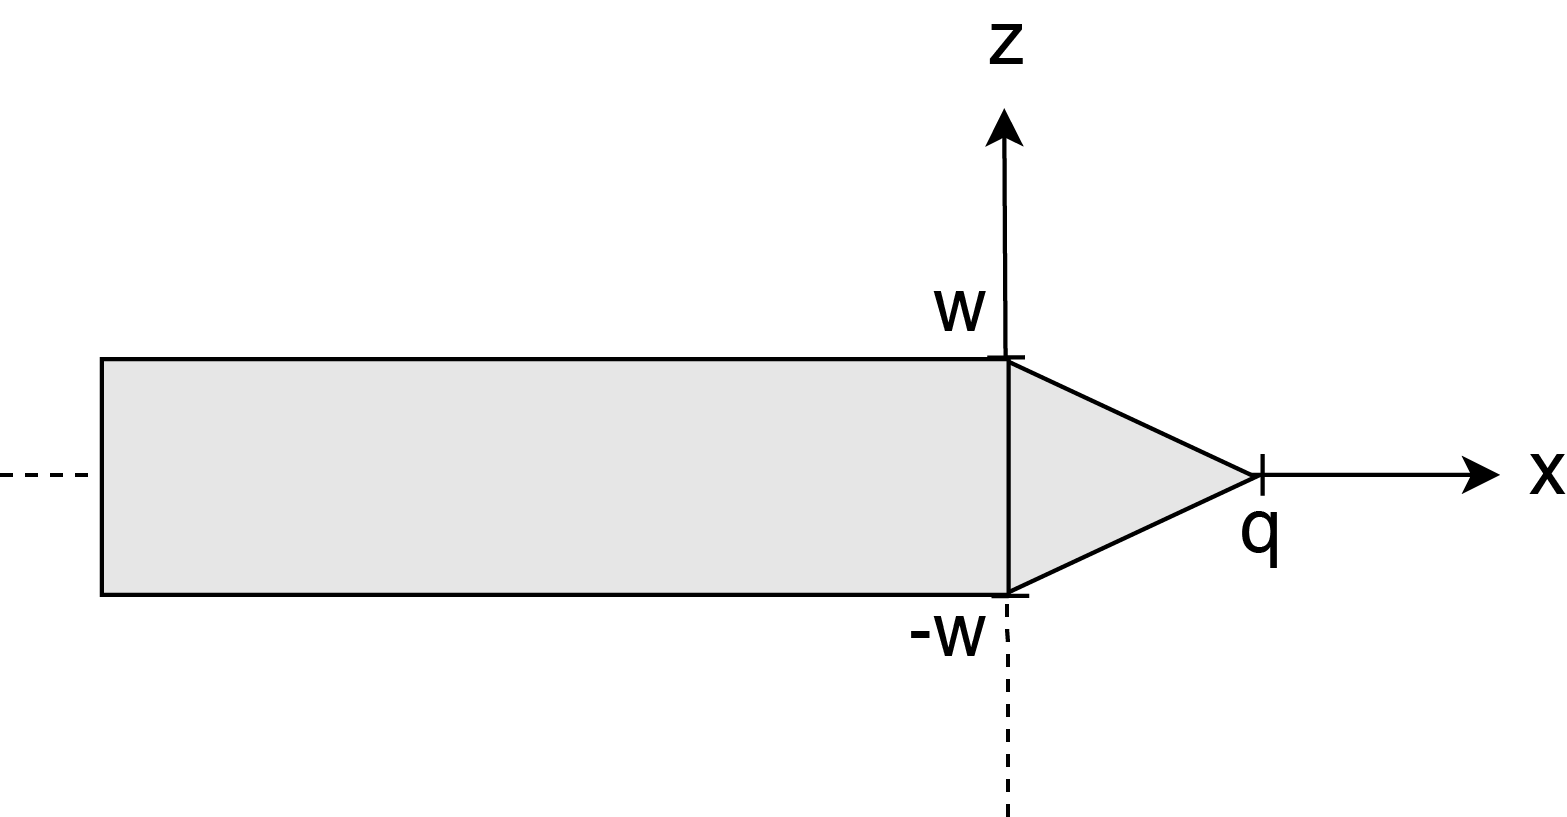
\includegraphics[width=0.4\textwidth]{figures/auv-geo}}
		\captionsetup{justification=centering,margin=2cm}
		\caption{Model of AUV used to calculate the LOS region}
		\label{fig:auv-geo}
	\end{figure}
	
	\item The regions for a $x \leq 0$ are defined as if the hydrophones were flat in the vehicle's surface, which leads to a simplified definition of the LOS region;
	
	\item Since hydrophone $r_1$ is integrated in every configuration, there is no necessity of defining its LOS region.

\end{itemize}

Having these relations into account, the LOS regions are then defined separately for $x \leq 0$ and $x > 0$. When $x \leq 0$, the second simplification previously mentioned is applied so all $ls_i$ are defined as the region greater/less or equal than the tangential to the position of hydrophone $i$ in plane yz. These tangential equations are defined in \ref{eq:los-s2} to \ref{eq:los-s9}.

\begin{eqnarray}
ls_2 \gets x \leq 0 \; \;  \wedge  \; \; z > r_{2_z} \\
\label{eq:los-s2}
ls_3 \gets x \leq 0 \; \;  \wedge  \; \; z < r_{3_z} \\
\label{eq:los-s3}
ls_4\gets x \leq 0 \; \;  \wedge  \; \; y > r_{4_y}  \\
\label{eq:los-s4}
ls_5\gets 	x \leq 0 \; \;  \wedge  \; \; y < r_{5_y} \\
\label{eq:los-s5}
ls_6 \gets	x \leq 0 \; \; \wedge  \; \; z \; \geq \; - y + w \sqrt{2} \\
\label{eq:los-s6}
ls_7 \gets	x \leq 0 \; \; \wedge  \; \; z \; \leq \; y - w \sqrt{2} \\
\label{eq:los-s7}
ls_8 \gets x \leq 0 \; \; \wedge  \; \;  z \; \geq \; y + w \sqrt{2} \\
\label{eq:los-s8}
ls_9 \gets 	x \leq 0 \; \; \wedge  \; \;  z \; \leq \; - y - w \sqrt{2}
\label{eq:los-s9}
\end{eqnarray}

By evaluating these equations, it is possible to infer that the LOS regions for $x \leq 0$ intersect each other, as illustrated in figure \ref{fig:los-color-s0}. The projection is correspondent to the yz plane with an inverted y-axis, in accordance with the previously presented model of the USBL system. Additionally, each colored line corresponds to the LOS region covered by the hydrophone with the same color. For instance, if a transmitter is located in $s_{cart}(-10,-10,-10)$, by analysis of the schematic it is observable that this position is covered by $ls_3$, $ls_5$ and $ls_9$, thus in line of sight of hydrophones 3,5 and 9.

\begin{figure}[!htbp]
	\makebox[\textwidth][c]{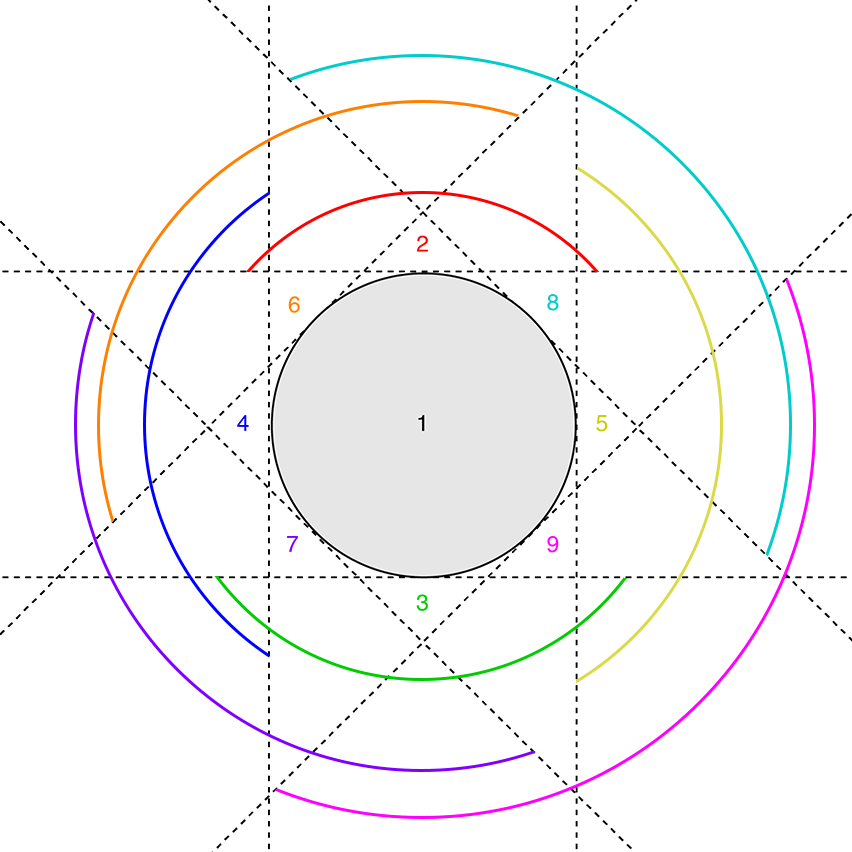
\includegraphics[width=0.6\textwidth]{figures/los-color-regions-back-crop}}
	\captionsetup{justification=centering,margin=2cm}
	\caption{Line of sight regions in plane yz for x < 0}
	\label{fig:los-color-s0}
\end{figure}

Analogously, when $x > 0$, all $ls_i$ are defined as the region greater/less or equal than the tangential to the position of hydrophone $i$ in planes xz or xy, depending on the hydrophone's location. Dealing with the hydrophones positioned in the y and z-axis, $r_2$, $r_3$, $r_4$ and $r_5$, it is possible to directly formulate equations that help defining $ls_2$, $ls_3$, $ls_4$ and $ls_5$ since the tangent plane to these hydrophones is perpendicular to referential planes. However, when considering hydrophones $r_6$, $r_7$, $r_8$ and $r_9$, which are not positioned in any referential axis, the tangential plane which passes through the hydrophone and the front limit of the cone is not parallel to any of the referential planes xy, xz or yz. Therefore, the equations that could define these planes require a rotation of the referential axis. In order to counter this issue, since the shape of the model projected in the yz plane is a circle , if hydrophones $r_6$, $r_7$, $r_8$ and $r_9$ are rotated a $45^{\circ}$ angle around the x-axis, they can become coincident with the positions of $r_2$, $r_4$, $r_5$ and $r_3$ respectively. Additionally, when considering this rotation, the position of the transmitter would also be rotated the same angle to maintain their relative positions. Overall, the used equations are defined by relations \ref{eq:los-b2} to \ref{eq:los-b5}, where the regarded $x,y,z$ coordinates are the original transmitter position for $ls_2$, $ls_3$, $ls_4$, $ls_5$, and the rotated transmitter position for $ls_6$, $ls_7$, $ls_8$, $ls_9$.

\begin{eqnarray}
ls_2, \;  ls_6  \gets x > 0 \; \;  \wedge  \; \; z \geq -\frac{w}{q} x + w  \\
\label{eq:los-b2}
ls_3, \;  ls_9 \gets x > 0 \; \;  \wedge  \; \; z \leq \frac{w}{q} x - w  \\
\label{eq:los-b3}
ls_4, \;  ls_7 \gets x > 0 \; \;  \wedge  \; \; y \geq -\frac{w}{q} x + w   \\
\label{eq:los-b4}
ls_5, \;  ls_8 \gets x > 0 \; \;  \wedge  \; \; y \leq \frac{w}{q} x - w  \\
\label{eq:los-b5}
\end{eqnarray}

After evaluating these equations and the limiting planes that they form, the projected regions of LOS for $r_2$, $r_3$, $r_4$ and $r_5$ are illustrated in \ref{fig:los-color-b0}, where their intersection is evident. The regions $ls_2$, $ls_3$, $ls_4$ and $ls_5$ are naturally similar to these, with an additional rotation of $45^{\circ}$ around the x-axis.

\begin{figure}[!htbp]
	\makebox[\textwidth][c]{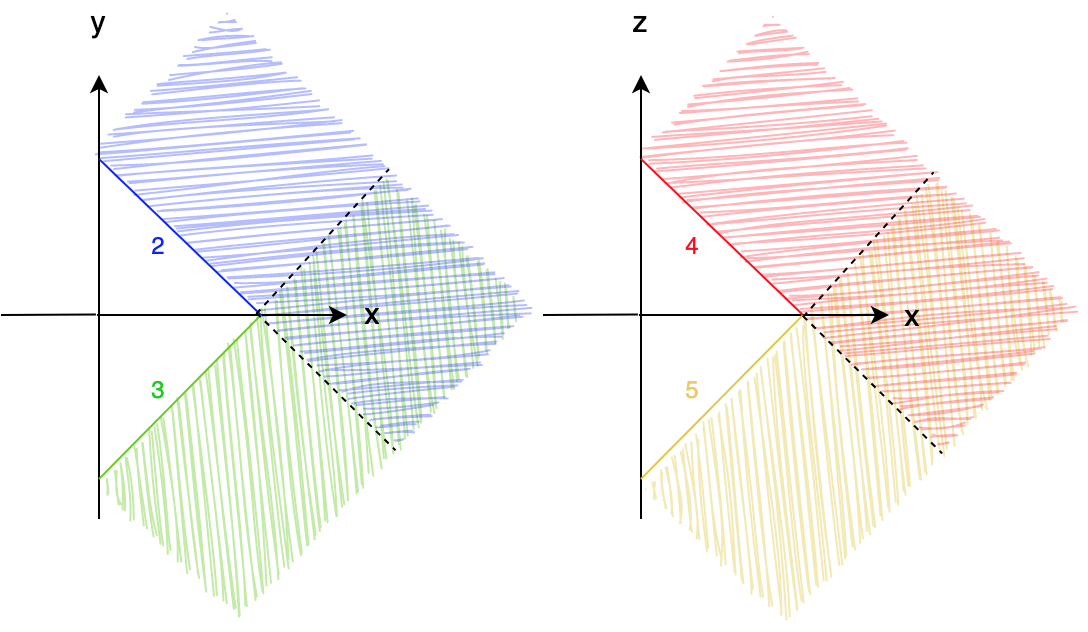
\includegraphics[width=0.7\textwidth]{figures/projections-los}}
	\captionsetup{justification=centering,margin=2cm}
	\caption{Line of sight regions in plane yx and zx for x $\geq$ 0}
	\label{fig:los-color-b0}
\end{figure}

In summary, it is possible to deduce that there is a larger quantity of different configurations that cover the space for $x>0$ than for $x \leq 0$ due to the model of the AUV and the considerations described in the course of this subsection. Therefore it is expected a better estimation for positions of the acoustic source with an azimuth angle between $-90^{\circ}$ and $90^{\circ}$.
%-------------------------------------------------------------------------
%\subsection{Limitations of the system}

%- considerations of the line of sight (mathematical approximations) - line of sight has to be defined for the model considered; if format changes, it has to be remade
%-------------------------------------------------------------------------

\section{Comprehensive study of geometric configurations performance} \label{sec:analysis_config_performance}

%Upon having full comprehension of the developed tool for determining the best configuration, it is interesting to compare its performance with widely used techniques. Therefore, the Crámer-Rao lower bound method was additionally implemented to do a systematic study on the performance of several hydrophone configurations.

For the purpose of demonstrating the functionality of the implemented system, various acoustic source positions were tested and the results analyzed.

The first demonstration evaluates the achieved MSE, azimuth deviation and elevation deviation for $s_{cart}(10,10,10)$. After simulating, plot \ref{fig:errors-101010} demonstrate the results, where the obtained parametric errors are illustrated for each of the 56 formulated configurations. Additionally, the configurations which are marked with a red circle correspond to those whose hydrophones all have full line of sight to the transmitter and the green star indicates which is the configuration that achieves the lowest error. The results of this experiment are aggregated in table \ref{tab:montecarlo-best1}. For the present case, the hydrophones considered to have line of sight to the target are $r_2$, $r_4$, $r_6$, $r_7$ and $r_8$. The configuration with lowest MSE and azimuth deviation is number 8, composed by hydrophones $r_1$, $r_2$, $r_4$ and $r_6$, which are the directly closer to the target. The configuration that originates lowest elevation deviation is number 19, composed by $r_1$, $r_2$, $r_7$ and $r_8$, which maximizes the baseline of the sensors with line of sight.

\begin{figure}[!htbp]
	\makebox[\textwidth][c]{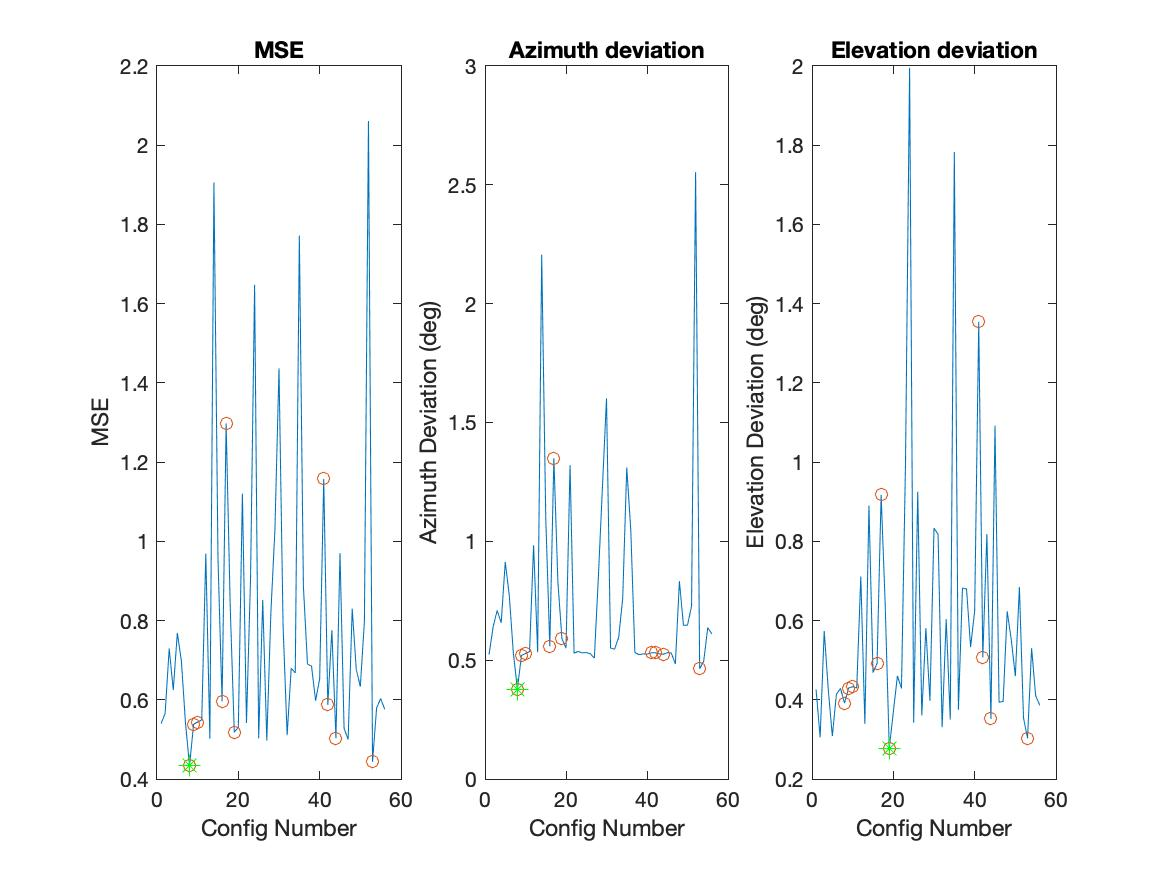
\includegraphics[width=1.3\textwidth]{figures/plot-[10,10,10]-1000s-errors}}
	\captionsetup{justification=centering,margin=2cm}
	\caption{Errors obtained for all configurations when estimating position $s_{cart}(10,10,10)$}
	\label{fig:errors-101010}
\end{figure}

Additionally, if the azimuth and elevation deviations are evaluated simultaneously, then the obtained plots can be overlaid to a clear comparison between results. Figure \ref{fig:both-101010} represents this situation where, as the label indicates, the azimuth deviation in degrees is represented by the blue line, the pink line is the elevation deviation in degrees, the red and green circles represent the configurations with line of sight to the target and the green star indicates, once again, the configurations which achieve the minimum deviations in azimuth and elevation. Additionally, the cyan diamond reveals which of the configurations leads to the minimum mean between the azimuth and the elevation deviations. In this case, this corresponds to configuration number 53 which reaches a mean deviation of 0.385 degrees. 

\begin{figure}[!htbp]
	\makebox[\textwidth][c]{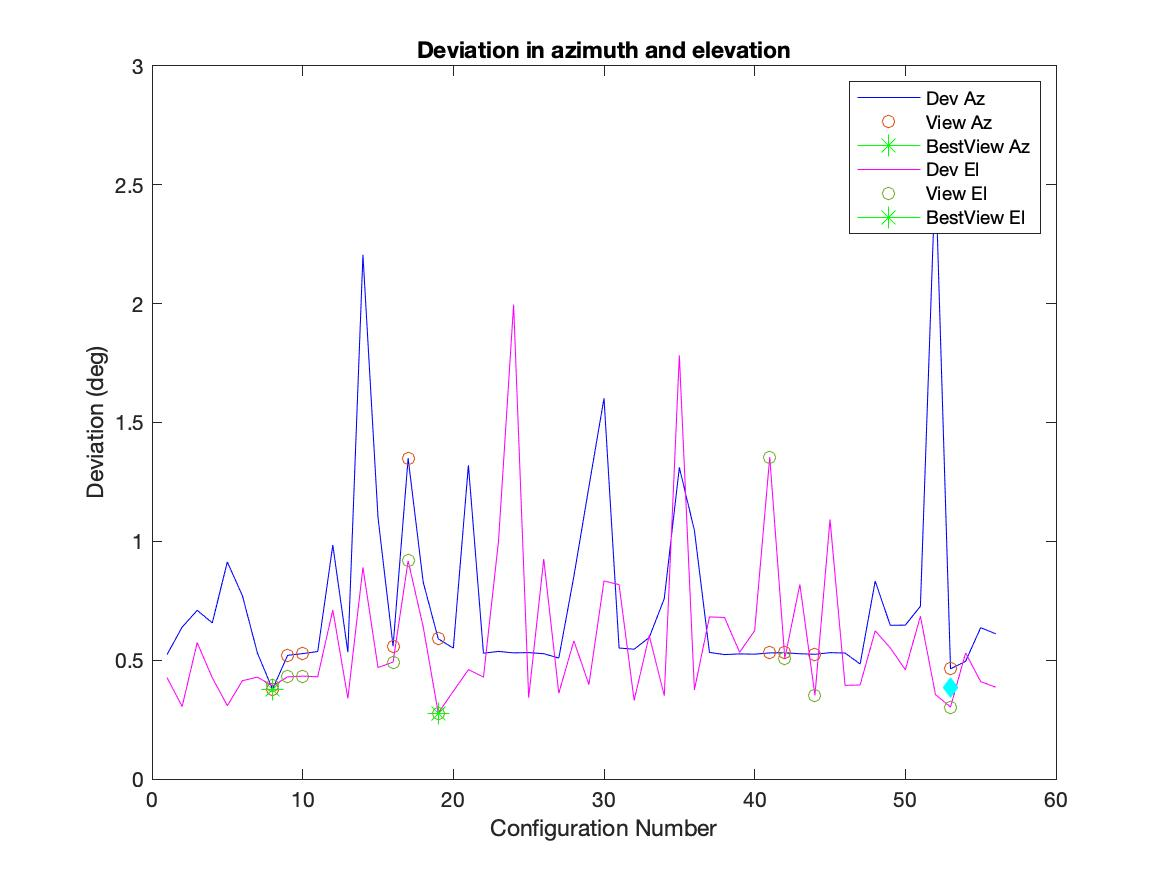
\includegraphics[width=0.9\textwidth]{figures/plot-[10,10,10]-1000s-both}}
	\captionsetup{justification=centering,margin=2cm}
	\caption{Overlaid azimuth and elevation deviations for all configurations when estimating position $s_{cart}(10,10,10)$}
	\label{fig:both-101010}
\end{figure}

In a second experiment, position $s_{cart}(100,100,100)$ is tested, which has the same azimuth and elevation angles as the previous position and a norm 10 times larger. For this case, the error range of azimuth and elevation estimation is approximately the same and the norm estimation presents an error around 10 times larger. Additionally, as expected the configurations that lead to the lowest errors are the same as for the first experiment.

A set of tests were executed in order to compare the performance of various positions estimation and to extract behavior patterns for the chosen configurations. The collected data is present in table \ref{tab:montecarlo-best1}, where the position of the transmitter are given in Cartesian coordinates by ($s_x$, $s_y$, $s_z$) and for each of the performance parameters it is presented the obtained best configuration number and the minimum error achieved by it. It should also be noted that the notation $0_{+}$/ $0_{-}$ indicates that for a theoretical position with a coordinate equal to zero it was returned a slightly positive/negative estimate of that same coordinate, due to the injected error.

\begin{table}[!htbp] %use H to adjust
	\begin{center}
		\begin{tabular}{ c c c |c c | c c | c c | c c }
			\toprule
			\multicolumn{3}{c|}{\textbf{$\bm{s_{cart}}$}} & \multicolumn{2}{c|}{\textbf{Azimuth}} & \multicolumn{2}{c|}{\textbf{Elevation}} & \multicolumn{2}{c|}{\textbf{Azimuth+Elevation}} & \multicolumn{2}{c}{\textbf{MSE}}   \\
			\midrule
			\multicolumn{1}{c}{$x$} & $y$ & $z$ & Config & Min  & Config & Min & Config & Min & Config & Min \\
			\midrule
			\multirow{1}{*}{10} & 10 & 10 & 8 & 0.377 & 19 & 0.278 &  53 & 0.385 & 8  & 0.434\\
			\midrule
			\multirow{1}{*}{-10} & -10 & -10 & 30 & 2.412 & 30 & 1.196 &  30 & 1.804 & 30  & 2.142\\
			\midrule
			\multirow{1}{*}{$0_{+}$} & -10 & -10 & 14 & 2.058 & 14 & 0.431 & 14 & 1.244  & 14  & 1.672 \\
			\midrule
			\multirow{1}{*}{100} & $0_{-}$ & $0_{-}$ & 47 & 0.177 & 32 & 0.177  & 11 & 0.284  & 11  & 0.330 \\
			\midrule
			\multirow{1}{*}{$0_{+}$} & 100 & $0_{+}$ & 9 & 0.596 & 16 & 0.425 & 16 & 0.512 & 16 & 0.586 \\
			\midrule
			\multirow{1}{*}{$0_{+}$} & $0_{-}$ & 100 & 37 & 52.572  & 39  & 0.381 & 37 & 26.479  & 39 & 32.602 \\
			\midrule
			\multirow{1}{*}{15} & -10 & 5 & 48 & 0.364 & 3 & 0.218 & 27 & 0.346 & 27 & 0.399 \\
			\bottomrule 
		\end{tabular}
		\caption{Summary of best configurations obtained by Monte Carlo simulation}
		\label{tab:montecarlo-best1}
	\end{center}
\end{table}

Some conclusions can be taken upon the analysis of these results: 
\begin{itemize}
	\item Configurations that achieve the overall minimum errors tend to integrate the LOS hydrophones that attain the larger baseline between them;
	
	\item Transmitter positions that return a higher number of LOS hydrophones, have more possible configurations to choose from and therefore can be more optimized, presenting the lowest errors;
	
	\item The points directly behind the AUV that cover positions with $y$ and $z$ in the range [-w,w], are not contained in any line of sight region;
	
	\item When the transmitter positions have $x \leq 0$, they are in line of sight of less hydrophones than for $x > 0$, so there are fewer possible configurations and the returned best option for the various parameters are more consistent. Consequently, the returned minimum errors are usually higher than for $x > 0$;
	
	\item Transmitter positions that are located near the y-axis, almost in parallel with the circle of hydrophones, are usually covered by only four LOS regions, which correspond to the sensors that are directly closer to the target;
	
	\item For elevation angles close to $90^{\circ}$ and $-90^{\circ}$, the azimuth deviation is much larger than at any other position as expected, since in that region the azimuth angle is more influenced by the injected errors leading to increased deviations.
\end{itemize}

\subsubsection{ Evaluation of the line of sight regions}	

Upon inspecting the overall obtained results and the whole function of the system, a particular analysis is conducted to the mechanism that defines the hydrophones' LOS regions. Therefore, after evaluating the position $s(10,10,10)$ that is expected to have an intermediate amount of hydrophones, two additional positions are tested.

The first position to be tested is $s(-10,-10,-10)$ which inherently has less hydrophones with line of sight, due to the method's limitation for $x \leq 0$. Additionally, since it is located in the seventh octant it is expected to be only in LOS with exactly three hydrophones, thus having only one available configuration with line of sight. After simulating, figure \ref{fig:errors-10-10-10} is obtained which verifies the concepts described. The only configuration with line of sight is number 30, composed by $r_1$, $r_3$, $r_5$ and $r_9$.

\begin{figure}[!htbp]
	\makebox[\textwidth][c]{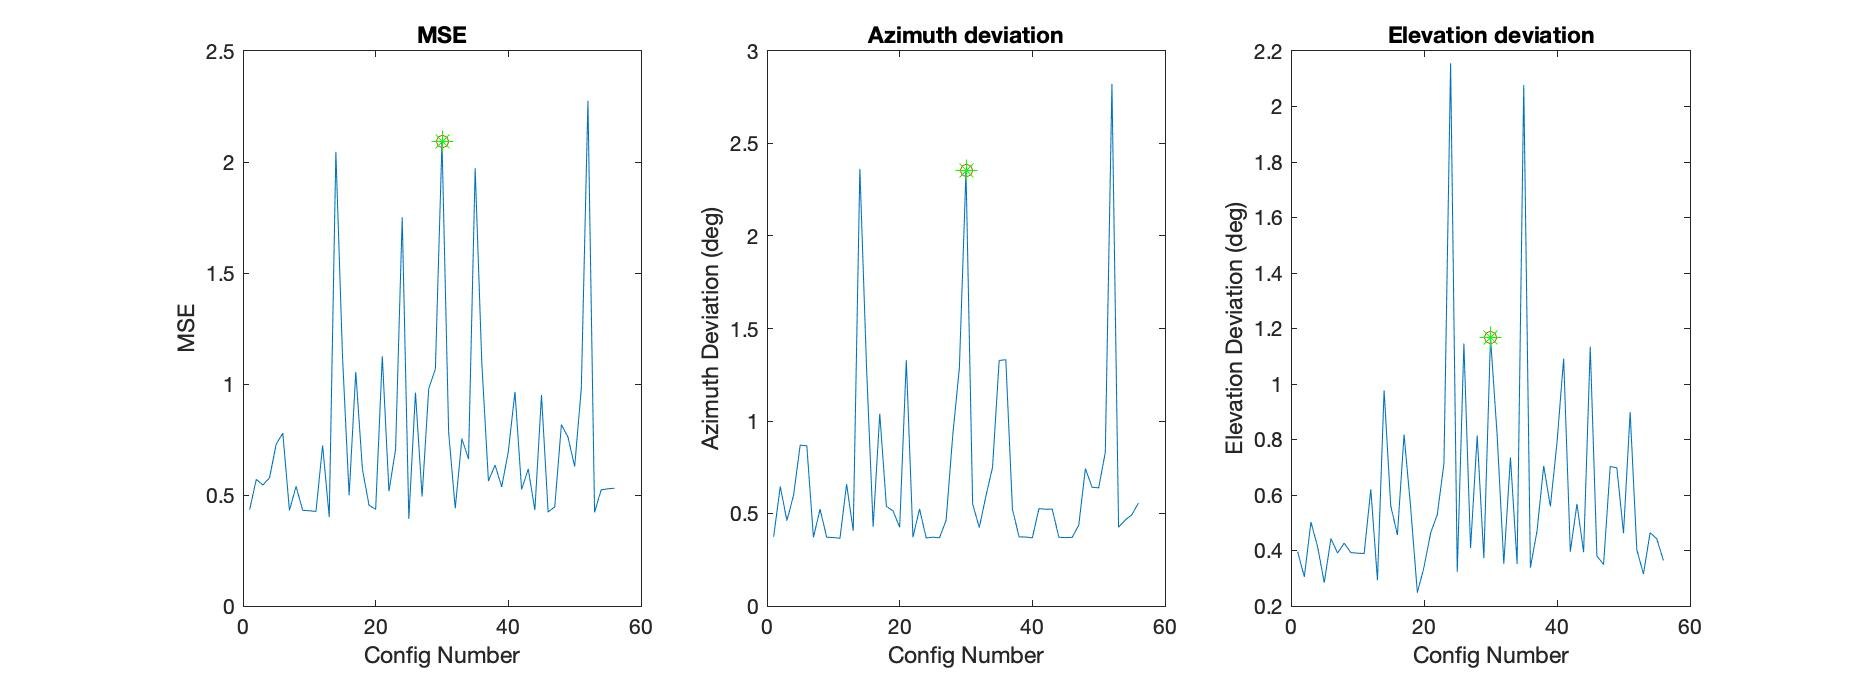
\includegraphics[width=1.3\textwidth]{figures/plot-[-10,-10,-10]-1000s-errors}}
	\captionsetup{justification=centering,margin=2cm}
	\caption{Errors obtained for all configurations when estimating position $s_{cart}(-10,-10,-10)$}
	\label{fig:errors-10-10-10}
\end{figure}

Then, position $s(100,0,0)$ is tested. Due to its long range location and the fact that it is assumed a conic shape at the front of the vehicle, it is expected that this point has line of sight for every employed hydrophone. Figure \ref{fig:errors-100-0-0} illustrates the simulated results which prove the theoretical expectation.

\begin{figure}[!htbp]
	\makebox[\textwidth][c]{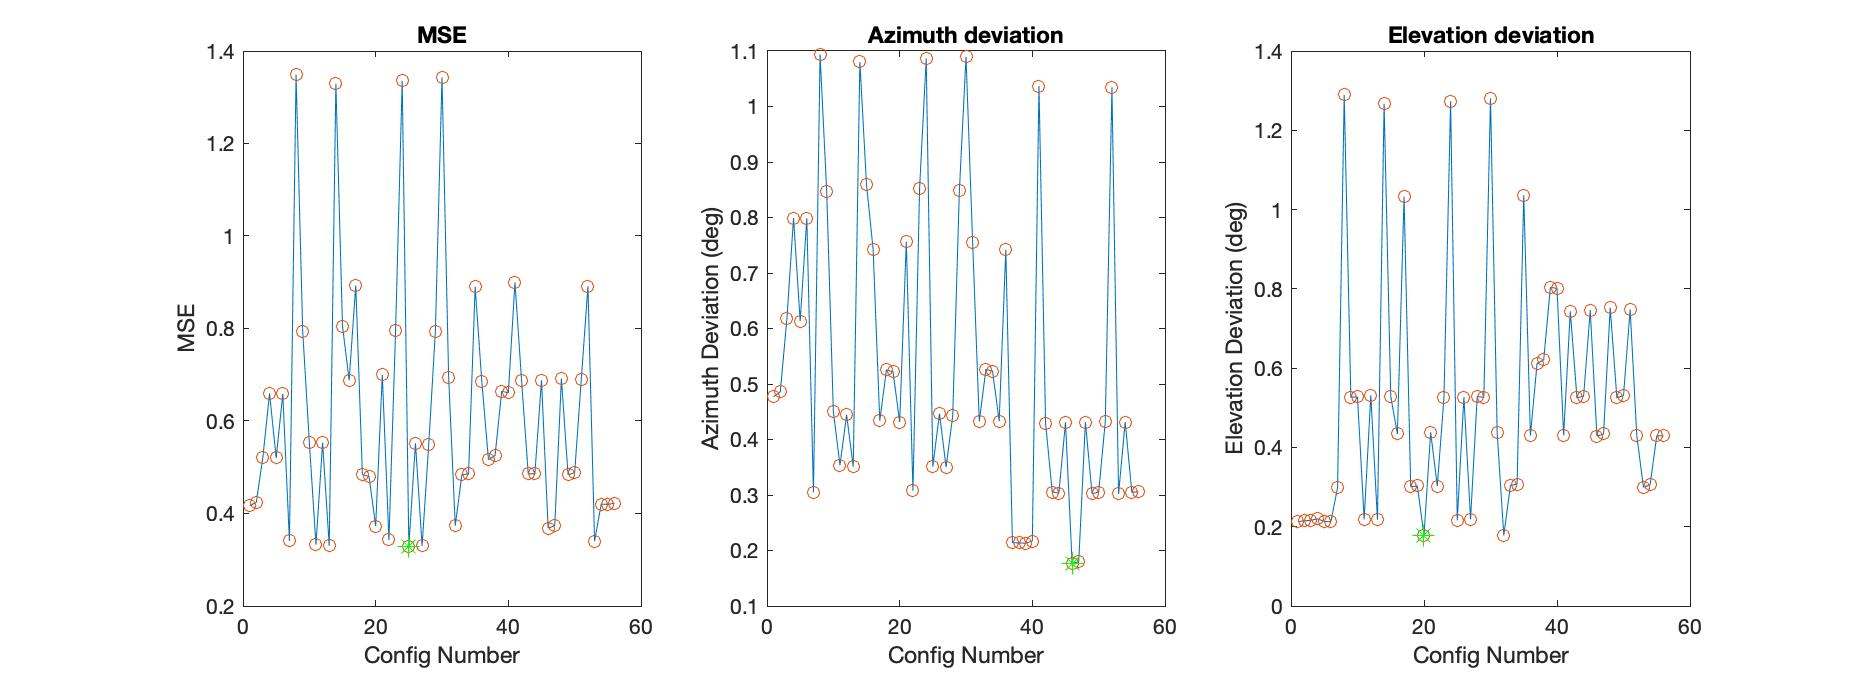
\includegraphics[width=1.3\textwidth]{figures/plot-[100,0,0]-1000s-errors}}
	\captionsetup{justification=centering,margin=2cm}
	\caption{Errors obtained for all configurations when estimating position (100,0,0)}
	\label{fig:errors-100-0-0}
\end{figure}

Lastly, an extensive verification process was held in order to ensure that the returned LOS hydrophones were plausible for many other positions. Table \ref{tab:LOS-var-pos} summarizes this search, containing a total of eleven positions spread over each octant and the reference axis. By consulting the hydrophone map illustrated in \ref{fig:9h-config}, it is possible to confirm that for every selected position the returned hydrophones are the logically expected.

\begin{table}[!htbp] %use H to adjust
	\begin{center}
		\begin{tabular}{ c c c c | c }
			\toprule
			\multicolumn{1}{c|}{} & \multicolumn{1}{c}{$s_x$} & $s_y$ & $s_z$ & Hydrophones with LOS\\
			\midrule
			\multicolumn{1}{c|}{x-axis} & \multirow{1}{*}{100} & 0 & 0 & 2, 3, 4, 5, 6, 7, 8, 9 \\
			\midrule
			\multicolumn{1}{c|}{y-axis} & \multirow{1}{*}{0} & 100 & 0 & 4, 6, 7 \\
			\midrule
			\multicolumn{1}{c|}{z-axis} & \multirow{1}{*}{0} & 0 & 100 & 2, 6, 8  \\
			\midrule
			\multicolumn{1}{c|}{$1^{st}$ octant} & \multirow{1}{*}{10} & 10 & 10 & 2, 4, 6, 7, 8 \\
			\midrule
			\multicolumn{1}{c|}{$2^{nd}$ octant} & \multirow{1}{*}{5} & 5 & -1 & 2, 3, 4, 6, 7 \\
			\midrule
			\multicolumn{1}{c|}{$3^{rd}$ octant} & \multirow{1}{*}{1} & -1 & 0 & 2, 3, 5, 8, 9  \\
			\midrule
			\multicolumn{1}{c|}{$4^{th}$ octant} & \multirow{1}{*}{1} & -10 & -10 & 3, 5, 7, 8, 9 \\
			\midrule
			\multicolumn{1}{c|}{$5^{th}$ octant} & \multirow{1}{*}{-100} & 10 & 10 & 2, 4, 6  \\
			\midrule
			\multicolumn{1}{c|}{$6^{th}$ octant} & \multirow{1}{*}{-1 } & 10 & -5 & 3, 4, 6, 7  \\
			\midrule
			\multicolumn{1}{c|}{$7^{th}$ octant} & \multirow{1}{*}{-1} & -1 & 1 & 2, 5, 8 \\
			\midrule
			\multicolumn{1}{c|}{$8^{th}$ octant} & \multirow{1}{*}{-1} & -100 & -10 & 3, 5, 8, 9 \\
			\bottomrule 
		\end{tabular}
		\caption{Hydrophones with line of sight for several $s$ positions}
		\label{tab:LOS-var-pos}
	\end{center}
\end{table}


\subsection{Comparison with Crámer-Rao lower bound}

Although the Monte Carlo approach and the Crámer-Rao bound method use distinct decision metrics,  it is still worth to understand the practical differences between the implementations regarding the developed dynamic reconfigurable method.

A simulation was performed in which position $s_{cart}(0,1000,0)$ is estimated by both methods, obtaining the estimate cloud by the Monte Carlo approach and the uncertainty axis in Crámer-Rao bound. Figure \ref{fig:compare-cramer-monte-0,1000,0-C} illustrates both data overlaid, using configuration C.

\begin{figure}[!htbp]
	\makebox[\textwidth][c]{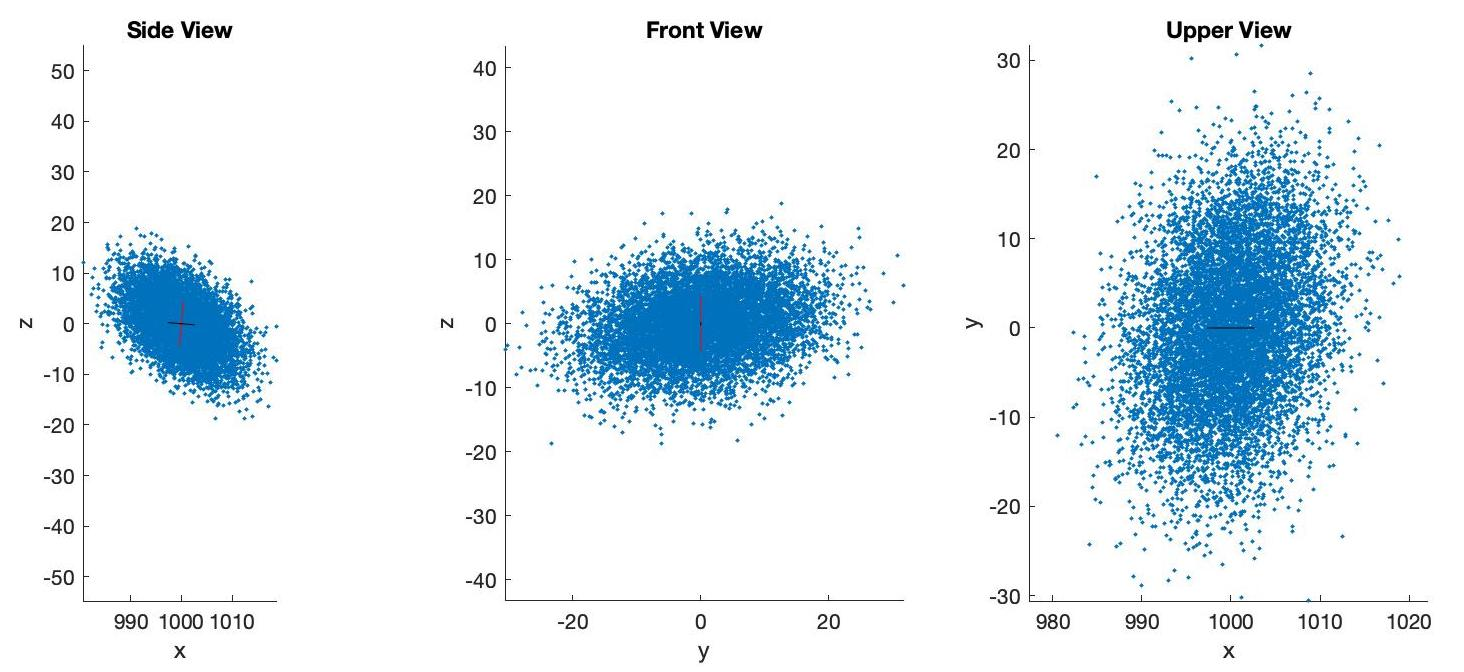
\includegraphics[width=1\textwidth]{figures/plot-fisher-monte-overlaid-0,1000,0-C}}
	\captionsetup{justification=centering,margin=2cm}
	\caption{Errors obtained for all configurations when estimating position (100,0,0)}
	\label{fig:compare-cramer-monte-0,1000,0-C}
\end{figure}

The plot reveals that the results are clearly not coherent, which is justified by the fact that the Crámer-Rao bound assumes any linear and unbiased estimator for the configuration's evaluation, while the Monte Carlo method is a non-linear estimator, due to the least squares equation that leads to the estimation in \ref{subsec:estimator}.

Therefore, to avoid lack of generalization, once more it is considered that the preferable mechanism to be used for analyzing the estimation accuracy is the FIM along with the desired optimality criteria.

\section{Optimal solution based on range} \label{subsec:opt-range}

After having a comprehensive understanding on the system that is capable of determining which is the best configuration of hydrophones to estimate a specific transmitter position, an alternate scenario can be explored. We now consider that the USBL system does not reconfigure which sensor configuration it should use in order to optimize the estimation  in real time. Instead, a performance study is conducted beforehand so that only two configurations are chosen to be deployed, corresponding to the ones which return the average best estimation of short and long range positions. This way, it would be possible to alternate which configuration is used depending solely on the distance to the target. Alternatively, it is also possible to define just one overall best configuration, in cases where there is the necessity of reducing the number of deployed hydrophones or if the two obtained configurations do not have a significant difference in performance.

In the development of this mechanism, there are some adjustments and similarities from the conditions established for the previous system. Firstly, it is assumed that the hydrophones are implemented in a structure shaped like an AUV with no physical form, thus all hydrophone positions have line of sight to any point in space. Additionally, the possibilities for the hydrophone locations are increased for a more extensive study. Once again, hydrophone $r_1$ is integrated in all configurations and a total of 24 possibilities are considered for the remnant three. These include the same 8 positions $r_2$ to $r_9$, established for the initial setup, to which are added positions $r_{10}$ to $r_{25}$ defined in table \ref{tab:config-25h}. This addition corresponds to two replicated circles from the initial one, that assume the same $y$ and $z$ coordinates but are deviated from each other a $d\_x$ equal to 20 centimeters. Figure \ref{fig:24h-config} illustrates all the considered possible positions for the hydrophone's deployment. Accordingly, the number of possibilities is not correspondent to combinations of three out of 24, $C(24,3)$, since these contain linearly dependent configurations, which correspond to hydrophones' positions that only differ in the $x$ coordinate. Therefore, the total number of available combinations is 1512.

\begin{table}[!htbp] %use H to adjust
	\begin{center}
		\makebox[\textwidth]{%
			\begin{tabular}{c | c c c c c c c c c c c c c c c c}
				\toprule
				& $r_{10}$ & $r_{11}$ & $r_{12}$ & $r_{13}$	& $r_{14}$ & $r_{15}$ & $r_{16}$ & $r_{17}$	& $r_{18}$ & $r_{19}$ & $r_{20}$ & $r_{21}$ & $r_{22}$ & $r_{23}$ & $r_{24}$ & $r_{25}$ \\ \midrule 
				\multirow{1}{0.5em}{x} 
				& 0 & 0 & 0 & 0 & 0 & 0 & 0 & 0 
				& $d\_x$ & $d\_x$ & $d\_x$ & $d\_x$ & $d\_x$ & $d\_x$ & $d\_x$ & $d\_x$\\
				\midrule 
				\multirow{1}{0.5em}{y} 
				& 0 & 0 & w & -w & e & e & -e & -e
				& 0 & 0 & w & -w & e & e & -e & -e\\
				\hline 
				\multirow{1}{0.5em}{z} 
				& w & -w & 0 & 0 & e & -e & e & -e
				& w & -w & 0 & 0 & e & -e & e & -e \\
				\bottomrule 
		\end{tabular}}
		\caption{Additional coordinates for an implementation with 25 hydrophones}
		\label{tab:config-25h}
	\end{center}
\end{table}

\begin{figure}[!htb]
	\makebox[\textwidth][c]{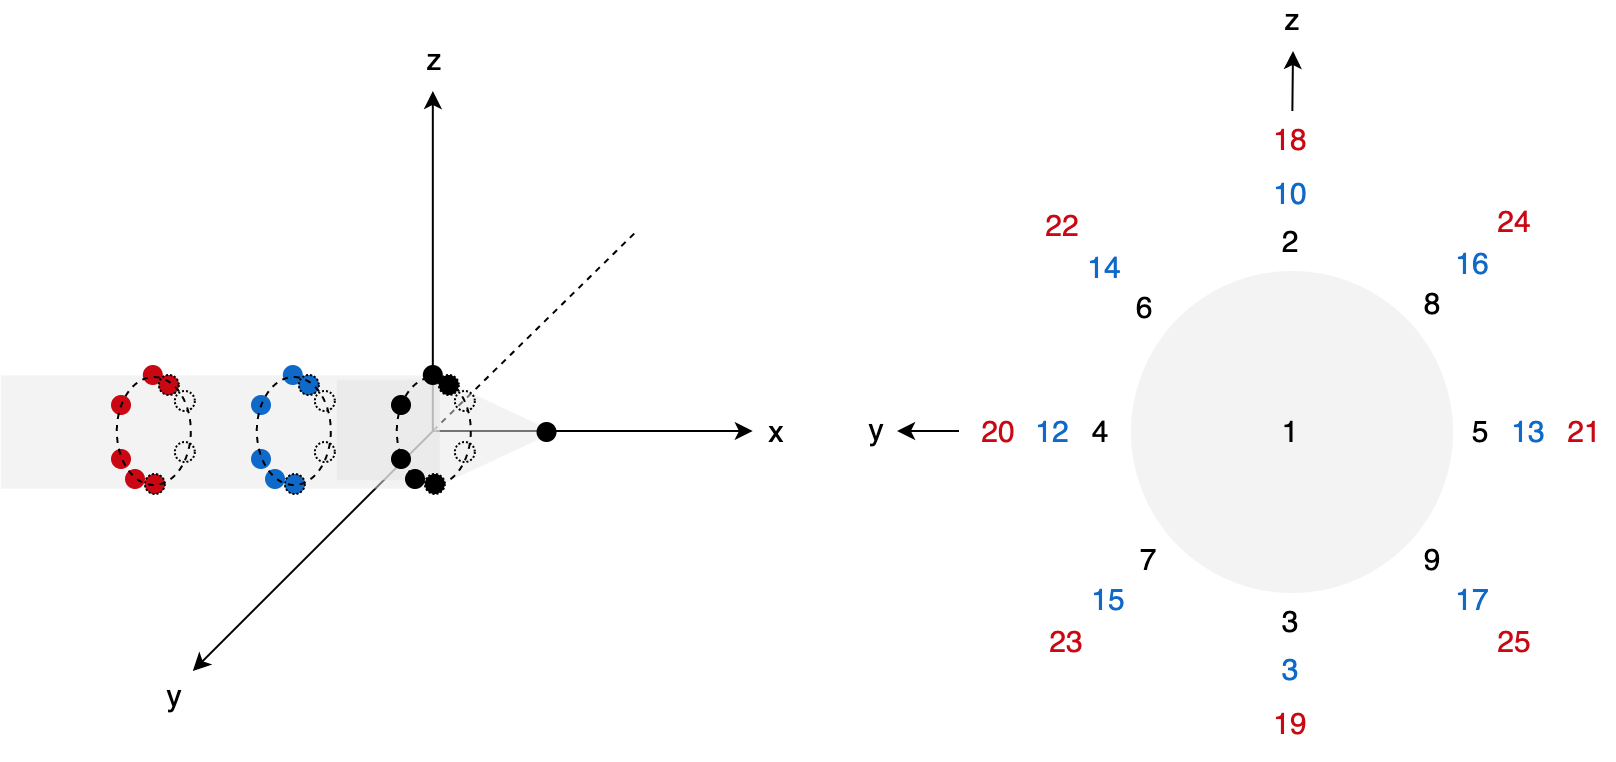
\includegraphics[width=0.9\textwidth]{figures/24h-config}}
	\captionsetup{justification=centering,margin=2cm}
	\caption{Hydrophone possible positions for optimality study based on range}
	\label{fig:24h-config}
\end{figure}

The applied algorithm is similar to the previously explained algorithms \ref{alg:alg1} and \ref{alg:alg2}, with the following variations:

\begin{enumerate}
	\item Similarly to the condition described in \ref{subsec:perform-compar-meth}, the acoustic source positions, $s$, to be estimated are defined in spherical coordinates, where for each defined norm, the elevation component covers the interval [-90$^{\circ}$ to 90$^{\circ}$] in steps of one and, for each elevation value, the azimuth component covers the interval [-180$^{\circ}$, 180$^{\circ}$] in steps of one, forming partial spheres around the reference axis' origin. The norm covers a range between 1 and 10000 meters.
	
	\item An additional logical loop is added in algorithm \ref{alg:alg1} between lines 1 and 2, so that for each possible configuration all $s$ are estimated a number of $i = 1000$ iterations.
	
	\item the $line\_of\_sight$ function is no longer used, as it is considered that all hydrophones have line of sight to every position $s$.
\end{enumerate}

From here it is possible to analyze which are the best returned configurations, according to the chosen parameters MSE, azimuth deviation, elevation deviation and combined azimuth and elevation deviations. According to the numeric errors that are obtained, it is then possible to decide whether there is a single configuration that has evidently a better performance than the others or if there is a pair of configurations that can be used to obtain individually better estimations for short and long range.

\subsection{Simulation results}

The previously defined method was tested through a series of simulations, in which all 1512 defined configurations repeatedly estimate all positions that compose spheres of defined norms. Then, the configurations that reveals lower estimation errors are selected as the most accurate in terms of azimuth angle, elevation angle, both angles simultaneously or MSE.

\begin{table}[!htbp] %use H to adjust
	\begin{center}
		\makebox[\textwidth]{%
			\begin{tabular}{ c | c c | c c | c c | c c}
				\toprule
				\multicolumn{1}{c|}{\textbf{}} & 
				\multicolumn{2}{c|}{\textbf{Azimuth}} & \multicolumn{2}{c|}{\textbf{Elevation}} & \multicolumn{2}{c|}{\textbf{Azimuth+Elevation}} & 
				\multicolumn{2}{c}{\textbf{MSE}}  \\
				\midrule
				\multicolumn{1}{c|}{Norm} & Config & Min  & Config & Min & Config & Min & Config & Min \\
				\midrule
				\multirow{1}{*}{1} & 792 & 0.4730 & 220 & 0.1758 & 862 & 0.3554 & 862 & 0.4654\\
				\midrule
				\multirow{1}{*}{2} & 792 & 0.4771 & 220 & 0.1738 & 827 & 0.3905 & 827 & 0.4549 \\
				\midrule
				\multirow{1}{*}{3} & 792 & 0.4820 & 220 & 0.1752 & 827 & 0.3921 & 860 & 0.4571\\
				\midrule
				\multirow{1}{*}{10} & 792 & 0.4796 & 260 & 0.1702 & 827 & 0.3918 & 827 & 0.4572\\
				\midrule
				\multirow{1}{*}{20} & 827 & 0.4893 & 260 & 0.1702 & 827 & 0.3905 & 827 & 0.4537\\
			%	\midrule
			%	\multirow{1}{*}{30} & 827 & 0.4875 & 260 & 0.1714 & 827 & 0.3913 & 827 & 0.4545\\
			%	\midrule
			%	\multirow{1}{*}{40} &  &  &  &  &  &  &  & \\
				\midrule
				\multirow{1}{*}{50} & 792 & 0.4940 & 220 & 0.1705 & 860 & 0.3947 & 860 & 0.4615\\
				\midrule
				\multirow{1}{*}{100} & 860 & 0.4881 & 260 & 0.1707 & 827 & 0.3913 & 860 & 0.4538\\
				\midrule
				\multirow{1}{*}{200} & 827 & 0.4853 & 260 & 0.1706 & 827 & 0.3889 & 827 & 0.4511\\
			%	\midrule
			%	\multirow{1}{*}{300} & 792 & 0.4879 & 260 & 0.1698 & 844 & 0.3937 & 844 & 0.4582\\
			%	\midrule
			%	\multirow{1}{*}{400} & 827 & 0.4864 & 260 &  0.1699 & 827 & 0.3883 & 827 & 0.4524\\
				\midrule
				\multirow{1}{*}{500} & 792 & 0.4886 & 260 & 0.1722 & 929 & 0.3935 & 862 & 0.4606\\
				\midrule
				\multirow{1}{*}{1000} & 827 & 0.4846 & 260 & 0.1709 & 827 & 0.3899  & 827 & 0.4524\\
				\midrule
				\multirow{1}{*}{10000} & 792 & 0.4810 & 260 & 0.1724 & 862 & 0.3920  & 827 & 0.4554\\
				\bottomrule 
		\end{tabular}}
		\caption{Results of Monte Carlo simulation for range based estimation}
		\label{tab:montecarlo-best-all}
	\end{center}
\end{table}

The overall results do not demonstrate a specific configuration to be the clear best in short or long range for the chosen parameters. In order to associate the obtained configuration numbers to the actual hydrophone placement, figure \ref{fig:config-images} gathers the most relevant representations for the simulations based on range. 

For performance based on azimuth, configuration number 792 shows best results for norms between 1 and 10 meters. However, for longer range the results do not tends to a specific configuration, alternating between three options. 

Regarding performance based on elevation, configuration 220 is indicated for 1 to 3 meters, while for ranges going from 10 to 10000 meters, configuration 260 is the clear preferred. As can be observed in the illustration, these are structurally similar.

When evaluating azimuth and elevation accuracy simultaneously or MSE, the results are not clear and many configurations are alternated, where number 827 is the most frequent.

Additionally, it should be noted that throughout all simulated norms, for each evaluated metrics the worse performance for every position corresponded to the same configurations.

\begin{figure}[!htb]
	\makebox[\textwidth][c]{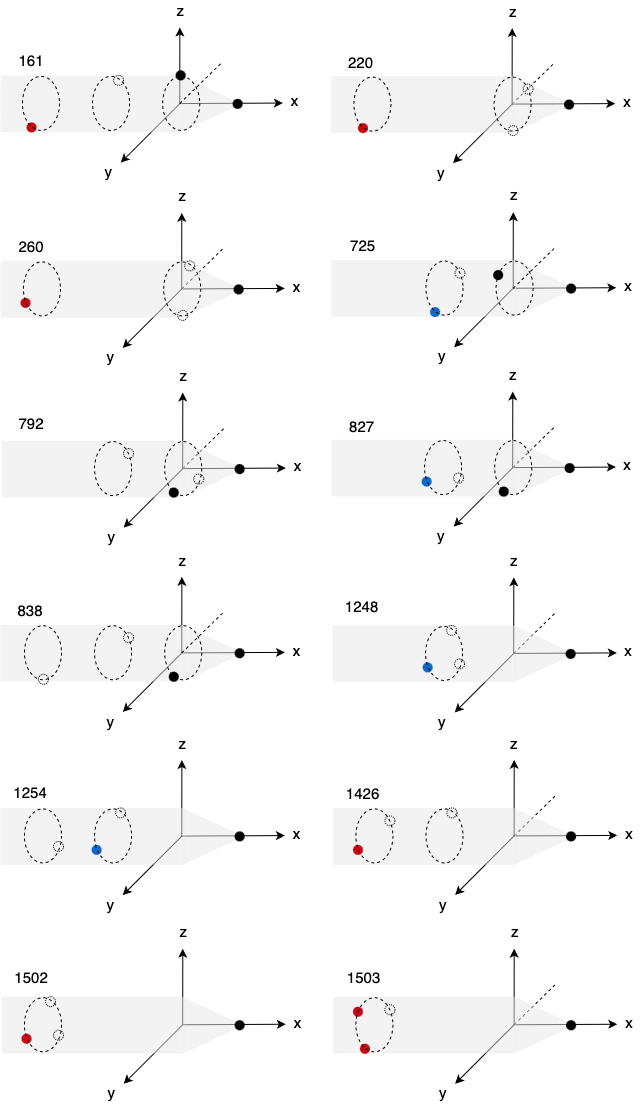
\includegraphics[width=0.8\textwidth]{figures/best-config-fim}}
	\captionsetup{justification=centering,margin=2cm}
	\caption{Illustration of relevant hydrophone configurations for range based estimation}
	\label{fig:config-images}
\end{figure}

To conclude, the obtained data do not show a clear tendency of two specific configurations being overall best for short and long range. This can be a result of the Monte Carlo simulation nature which originates results that do not have a clear sequence as expected. Therefore, this same experiment is repeated in the next subsection using the Fisher Information Matrix integrated in the Crámer-Rao bound method.

\subsection{FIM simulation}

Since the Fisher Information Matrix is a reliable and well know tool for evaluating a configuration's performance, then a simulation was executed for determining the best configuration for short and long range estimations.
Therefore, the method was integrated in a Monte Carlo approach that tests all 1512 configurations defined previously described in this section, which integrate a total of 25 different hydrophones. For each configuration, all $s$ positions that make up a sphere with a defined norm are used to calculate the FIM and evaluate the desired criteria. Among all, the configurations that demonstrate the preferred results correspond to the best performance in each specific criteria.

Table \ref{tab:fim-best1} summarizes the obtained results for a norm range between 1 and 10000 meters. A standard metric and three optimality criteria were observed and for each of them, the table indicates the configuration number that proved to have the best performance and the respective achieved values: 

\begin{itemize}
	\item In E-optimality, the Eigenvalue column contains the minimum larger eigenvalue found among all configurations
	
	\item In D-optimality, the Determinant column includes the minimum computed determinant of the inverse of the FIM for all configurations
	
	\item In A-optimality, the Trace column comprises the minimum sum of eigenvalues of the FIM among all configurations
\end{itemize}

\begin{table}[!htbp] %use H to adjust
	\begin{center}
		\makebox[\textwidth]{%
		\begin{tabular}{ c | c c | c c | c c }
			\toprule
			\multicolumn{1}{c|}{\textbf{}} & 
			\multicolumn{2}{c|}{\textbf{E-optimality}} & \multicolumn{2}{c|}{\textbf{D-Optimality}} & \multicolumn{2}{c|}{\textbf{A-Optimality}} \\
			\midrule
			\multicolumn{1}{c|}{Norm} & Config & Eigenvalue  & Config & Determinant & Config & Trace \\
			\midrule
			\multirow{1}{*}{1} & 1248 & 6.2$\times10^{-3}$ & 1503 & 1.6$\times10^{-3}$ & 600 & 2.3$\times10^{-5}$ \\
			\midrule
			\multirow{1}{*}{2} & 1248 & 0.012 & 1503 & 2.5$\times10^{-3}$ & 1426 & 9.2$\times10^{-5}$  \\
			\midrule
			\multirow{1}{*}{3} & 1248 & 0.018 & 1503 & 3.3$\times10^{-3}$ & 1426 & 2.1$\times10^{-4}$  \\
			\midrule
			\multirow{1}{*}{10} & 1502 & 0.061 & 1503 & 7.4$\times10^{-3}$ & 1426 & 2.4$\times10^{-3}$ \\
			\midrule
			\multirow{1}{*}{20} & 1502 & 0.121 & 1503 & 0.012 & 1426 & 9.6$\times10^{-3}$\\
		%	\midrule
		%	\multirow{1}{*}{30} & 1502 & 0.182 & 1503 & 0.015 & 1426 & 0.022 & 68 & 9.1$\times10^{-4}$ \\
		%	\midrule
		%	\multirow{1}{*}{40} & 1502 & 0.242 & 1503 & 0.019 & 1426 & 0.039 & 68 & 1.1$\times10^{-3}$ \\
			\midrule
			\multirow{1}{*}{50} & 1502 & 0.303 & 1503 & 0.022 & 1426 & 0.061   \\
			\midrule
			\multirow{1}{*}{100} & 1502 & 0.061 & 1503 & 0.034 & 1426 & 0.242 \\
			\midrule
			\multirow{1}{*}{200} & 1502 & 1.212 & 1503 & 0.054 & 1426 & 0.968  \\
		%	\midrule
		%	\multirow{1}{*}{300} & 1502 & 1.818 & 1503 & 0.071 & 1426 & 2.180 & 68 & 4.2$\times10^{-3}$  \\
		%	\midrule
		%	\multirow{1}{*}{400} & 1502 & 2.424 & 1503 & 0.087 & 1426 & 3.875 & 68 & 5.1$\times10^{-3}$  \\
			\midrule
			\multirow{1}{*}{500} & 1502 & 3.029 & 1503 & 0.100 & 1426 & 6.055  \\
			\midrule
			\multirow{1}{*}{1000} & 1502 & 6.059 & 1503 & 0.159 & 1426 & 24.226 \\
			\midrule
			\multirow{1}{*}{10000} & 1502 & 60.587 & 1503 & 0.737 & 1426 & 2.42$\times10^{3}$ \\
			\bottomrule 
		\end{tabular}}
		\caption{Results of FIM simulation for range based estimation}
		\label{tab:fim-best1}
	\end{center}
\end{table}

The overall results do not demonstrate a specific configuration to be the clear best in short or long range for the chosen parameters. In order to associate the obtained configuration numbers to the actual hydrophone placement, figure \ref{fig:config-images} gathers the most relevant representations for the simulations based on range. 

By inspection, it is possible to understand that for each criterion there is a clear best configuration for short and long range. The hydrophone placement of the mentioned configuration numbers are illustrated in figure \ref{fig:config-images} for a more practical interpretation. 

Therefore, in terms of E-optimality configuration, an approximately constant error of 0.6\% is visible, where number 1248 shows the best performance for range between 1 and 3 meters, while from 10 to 10000 meters configuration 1502 is considered the best.

For D-optimality, a single configuration, number 1503, was considered the best for all defined ranges, which corresponds to an hydrophone placement that maximizes the baseline between the fixed sensor and the other three.

Finally, in terms of A-optimality configuration number 600 is indicated for norm equal to 1 meters and, for the remaining ranges, number 1426 is chosen as the preferable option.

\section{Summary and Discussion}

\note{escrever melhor, reunir mais ideias}


Considering that the E-optimality is the most relevant criterion for this application, two configurations could be deployed, 1248 for short range and 1502 for long range, achieving an approximately constant error of 0.6\%.

This system can be applied to a dynamic reconfigurable configuration mechanism that allows the USBL system to be optimized in real time .
